\section{PIR协议与应用框架设计}
针对上述问题,本文提出了一套相对应的解决方案。具体来说,本文提出了一套高性能的亚线性复杂度PIR协议,能够以较低的代价生成计算证明,从而确保服务的可靠性。同时,本文还设计了一个可拓展的PIR框架,使得PIR服务能够轻松实现横向扩展和容灾。最后,本文深入探讨了这一框架在区块链中的应用。
\subsection{高性能可验证的PIR协议}
本文分析了先前研究中出现的“虚构查询”问题,用户需生成大量虚假查询以维护服务的隐私性。虚构查询的存在不仅导致服务提供商进行了大量无效计算,降低了查询效率,同时也导致服务隐私性无法保证,为攻击者提供了攻击突破口。我们详细研究了“虚构查询”和“选择失败攻击”之间的关系,阐明了当前基于“虚构查询”的PIR协议易受“选择失败攻击”攻击的原因。

为解决这一问题,我们提出了一种无需虚构查询的亚线性复杂度PIR协议,改进了在线查询方式,优化了具体参数,使得在线查询效率相较于当前行业领先工作\cite{C:LazPap23,Piano}提高了6-7倍。该协议使用伪随机函数代替了可穿孔伪随机函数,省去了昂贵的穿孔构造;利用数据库划分加速集合隶属测试,并使用一种全新的$Hint$构造解决了协议正确性与隐私性问题。我们提供了该协议的多服务器构造与单服务器构造,同时还提出了一种融合多服务器构造与单服务器构造优点的执行模型,该模型在在线计算中无需多服务器参与,同时兼顾了离线计算量,代价是需要一定额外存储空间。

为解决可验证性问题,该协议借鉴外包计算的验证过程,采用隐藏参数与重复计算的方式进行验证。通过在$Hint$中增加额外用于验证的信息,客户端能够在在线阶段使用这些信息验证服务器的答案。这种验证方式是可选的,若不需要验证过程,客户端可以不使用,甚至完全不获取这些额外信息。这使得该协议适用于多种应用场景,根据需求可选择是否使用验证过程。

\subsection{可拓展PIR框架}

\begin{figure}
    \centering
    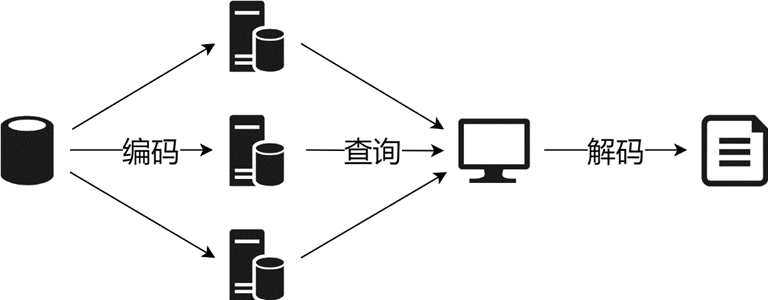
\includegraphics[width=0.8\textwidth]{figure/PIR-framework.png}
    \caption{PIR框架}
    \label{fig:pir-framework}
\end{figure}

针对PIR的存储和扩展性问题,本文提出了一种基于编码的PIR框架。如图 \ref{fig:pir-framework} 所示,该框架允许服务提供者将数据库通过编码拆分成多个较小规模的数据库,然后将这些小数据库分别部署在不同的物理设备上。这些物理设备将独立运行PIR协议,作为一个整体向客户端提供PIR服务,充分利用多台设备的存储和计算能力。客户端通过解码获得查询结果。这样一来,PIR服务不再受单台物理设备的内存限制,能够通过横向拓展来不断扩展,以适应更大规模的数据库。

同时,通过纠错码的纠错能力,这一框架允许服务提供者通过冗余保障PIR服务的可用性。在这一框架中,如果底层协议具有可验证性,纠错码就可以特化为纠删码,从而实现更高的编码利用率。本文注意到在这一框架中,如果底层协议不要求服务器使用私有参数,客户端所提出的查询就可以重复利用,由一台代理服务器进行转发,从而将框架在两方面进行优化:

\begin{enumerate}
    \item \textbf{使分布式性质透明}:客户端不需要了解各分布式设备的地址,只需要向代理服务器发起请求即可
    \item \textbf{降低通信量}:通过服务器转发的方式,客户端通信量随服务器数量增长而减小。同时,多台服务器在物理空间上紧密连接时,转发可以充分利用这一点,降低总传输成本。
\end{enumerate}

结合本文提出的PIR协议,这一框架使得PIR服务更加高效可靠。

\subsection{基于区块链的应用}

\begin{figure}
    \centering
    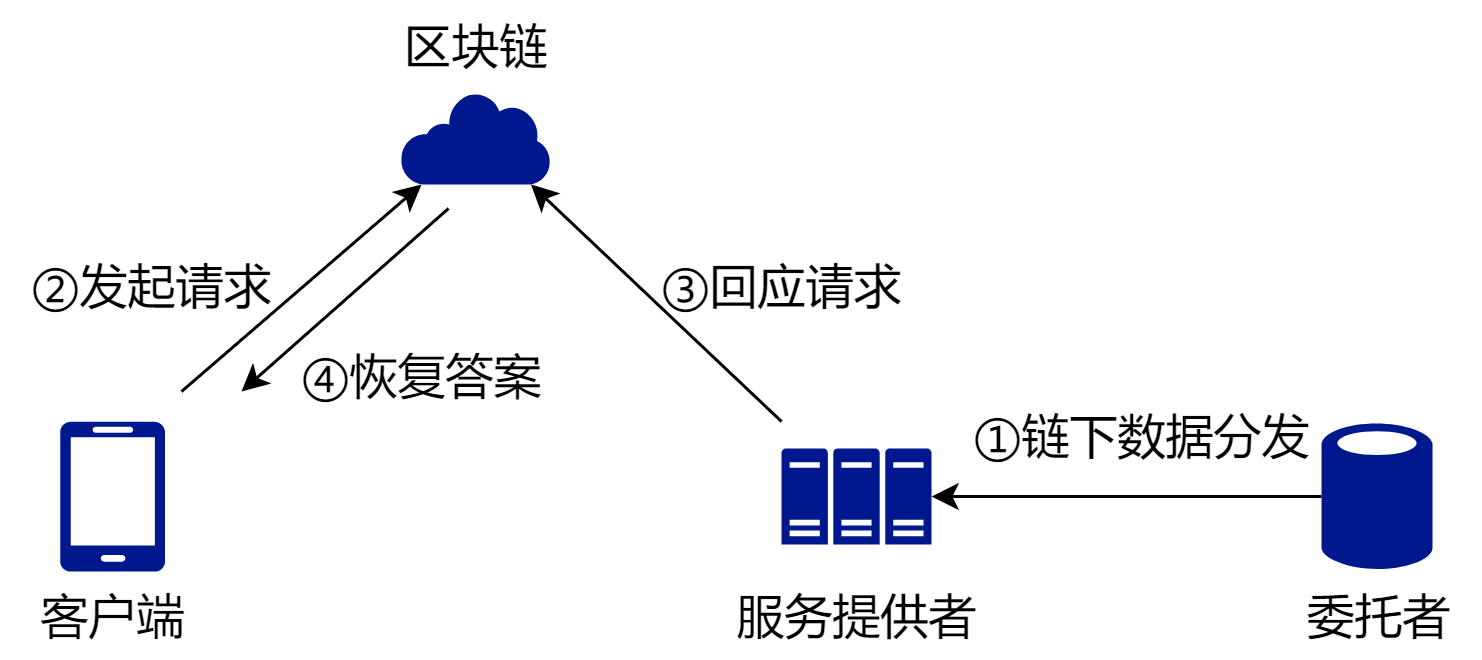
\includegraphics[width=0.8\textwidth]{figure/区块链应用模型.png}
    \caption{区块链应用模型}
    \label{fig:pir-application}
\end{figure}
本文将这一框架运用于“\projectname”课题中,针对黑名单匹配与用户隐私保护问题提出了基于PIR的解决方案,将协议验证流程转化为智能合约,实现公开验证。具体方案如图\ref{fig:pir-application}所示:委托者与服务提供者先达成协议,并通过链下分发数据库;客户端通过区块链上的智能合约发起查询请求;服务提供者通过智能合约提供服务。利用PIR的公开性和抗监听特性,这一方案天然与区块链相契合。通过智能合约实现请求过程的原子化,保护客户端和服务提供者权益。利用PIR框架的可靠性,这一方案可容忍服务提供者掉线、网络硬件故障等问题,提供持续服务。查询、验证、纠错等功能集中在一个智能合约中,极大简化了客户端使用PIR服务的流程。